\documentclass[letterpaper,12pt]{article}

\usepackage{tabularx} % extra features for tabular environment
\usepackage{amsmath}  % improve math presentation
\usepackage{amssymb}
\usepackage{multirow}
\usepackage{xcolor}
\usepackage{gensymb}
\usepackage{appendix}
\usepackage{bigints}

\usepackage{gensymb}
\usepackage{float}
\usepackage{listings}
\usepackage[export]{adjustbox}
\usepackage{graphicx} % takes care of graphic including machinery
\usepackage[margin=1in,letterpaper]{geometry} % decreases margins
\usepackage{cite} % takes care of citations
\usepackage[final]{hyperref} % adds hyper links inside the generated pdf file
\newcommand*{\tran}{^{\mkern-1.5mu\mathsf{T}}}

\hypersetup{
    colorlinks=false,       % false: boxed links; true: colored links
    linkcolor=blue,        % color of internal links
    citecolor=blue,        % color of links to bibliography
    filecolor=magenta,     % color of file links
    urlcolor=blue         
}
%++++++++++++++++++++++++++++++++++++++++++++++++++++++++++++++++++++++++++++++++



%++++++++++++++++++++++++++++++++++++++++++++++++++++++++++++++++++++++++++++++++
% Start modifying the labwork number, your team number and the name and METU id
% of your group members.
\newcommand{\reporttitle}{Solution Set 4}
\newcommand{\reportauthor}{ Volkan Aydıngül (Id: 0075359 )\\
                            }
                            % If any teammate does not help to write this report,
                            % you may not write his/her name here.
%++++++++++++++++++++++++++++++++++++++++++++++++++++++++++++++++++++++++++++++++



%++++++++++++++++++++++++++++++++++++++++++++++++++++++++++++++++++++++++++++++++
% DO NOT MODIFY THIS SECTION
\begin{document}
\begin{titlepage}
\newcommand{\HRule}{\rule{\linewidth}{0.5mm}}
\begin{center} % Center remainder of the page
%	LOGO SECTION

\includegraphics[width = 8cm]{figures/koc_logo.png}

%	HEADING SECTIONS
\textsc{\Large PHYS 514 - Computational Physics}\\[1.5cm] 
%	TITLE SECTION
\HRule \\[0.6cm]
{ \huge \bfseries \reporttitle}\\ % Title of your document
\HRule \\[1.5cm]
\end{center}
\vspace{2cm}
%	AUTHOR SECTION
\begin{flushleft} \large
\textit{Author:}\\
\reportauthor% Your name
\end{flushleft}
\vspace{2cm}
\makeatletter
Date: \@date 
\vfill % Fill the rest of the page with whitespace
\makeatother
\end{titlepage}
%++++++++++++++++++++++++++++++++++++++++++++++++++++++++++++++++++++++++++++++++




\tableofcontents
\newpage





%\begin{figure}[H] 
%   \centering \includegraphics[width=\columnwidth]{figures/figure.png}           
%                \caption{Caption}                
%                   \label{fig:label}
%   \end{figure}

\section{Problem XI}

\subsection{General Looking of the Data}
\begin{figure}[H]
    \centerline{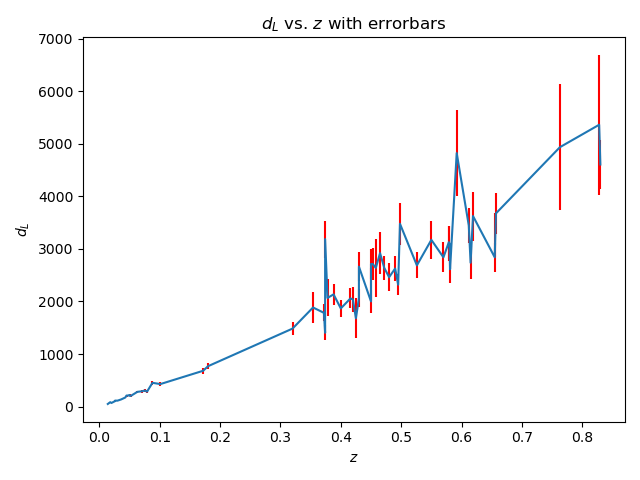
\includegraphics[width=\linewidth]{figures/errorplot.png}}
    \caption{Errorbar Plot of the Data}
    \label{fig:errorplot}
    \end{figure}
\paragraph{}In Figure \ref{fig:errorplot}, the general trend of the data can be observed and the errors in the measurement can be investigated.

\subsection{Linear Fit on the Data}
\paragraph{} In Figure \ref{fig:linfit}, the linear fitting process executed on the data can be observed. The fitting scheme is following:
\begin{equation*}
    d_L = az+b
\end{equation*}
where $z$ represents the independent variable  (redshift parameter), $d_L$ represents the dependent variable (luminosity distance of the source). The purpose was to obtain $a$ and $b$ for the condition of $z<0.1$.
\paragraph{} In the problem set, also, the cosmological term called \textit{Hubble length} is asked. It is known that:
\begin{equation*}
    d_L = d_Hz
\end{equation*}

%%% ! REFERENCE

where $d_H$ is the \textit{Hubble length}.
\paragraph{} According to the above notion, one can easily expect that, as a result of linear fitting, $a$ should result in approximately $d_H$ and $b$ should be result in approximately $0$. From Figure \ref{fig:linfit}, it can be displayed that:
\begin{equation*}
    d_H = a = 4508.135
\end{equation*}
and $b$ is relatively close to $0$.

\begin{figure}[H]
    \centerline{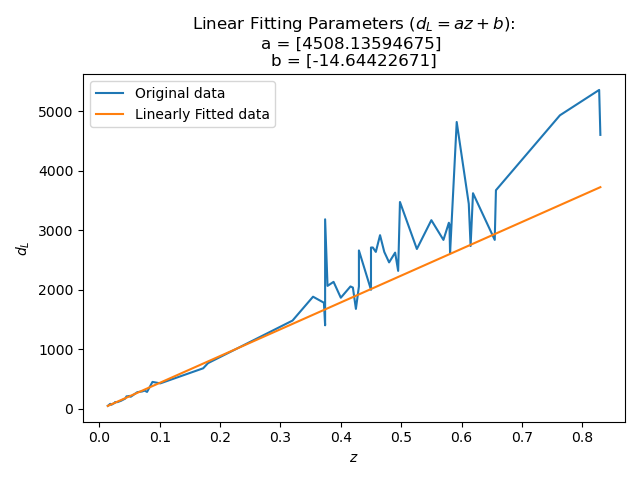
\includegraphics[width=\linewidth]{figures/linfit.png}}
    \caption{Linear Fit on the Data}
    \label{fig:linfit}
    \end{figure}

\subsection{Nonlinear Fit on the Data}
\paragraph{} In many cases, it is obvious that the linear fit does not result in fairly satisfying results. In this case, nonlinear fitting is the option that one should choose. In this context, the objective function is following:
\begin{equation*}
    d_L = (1+z)d_H \int_{0}^{z} \frac{1}{\sqrt{\Omega_M(1+x)^3 + (1-\Omega_M)}} \,dx 
\end{equation*}
wihch can be also represented as:

\begin{equation*}
    f(z, d_H, \Omega_M) = d_L = (1+z)d_H I(z, \Omega_M)
\end{equation*}
where $z$ are independent variable and $d_L$ is the dependent variable. Also, it should be noted that $\Omega_M$ is normalized form of matter density in the universe. To solve nonlinear fitting problem, there exists several methods. One method can be the transformation of the problem into nonlinear root finding problem. The procedure will be explained in following statements.
\paragraph{} First, an objective function should be defined, which can be observed below:
\begin{equation*}
    J = \sum_{k=1}^{n} \left((f_k(z, d_H, \Omega_M) - \hat{{d_L}_k} \right)^2
\end{equation*} 

As in the case of all optimization problem, the purpose is to minimize above equation to get optimal parameters. However, the important point is that the minimization should be with respect to $d_H$ and $\Omega_M$, since the main objective is to find them. Therefore, the derivative with respect to these variables should be computed, which can be observed below:
\begin{equation*}
    \frac{\partial J}{\partial d_H} =\sum 2 \left((1+z)d_H I(z, \Omega_M) -d_L\right)(1+z)I(z, \Omega_M) = 0
\end{equation*}

\begin{equation*}
    \frac{\partial J}{\partial \Omega_M} =\sum 2 \left((1+z)d_H I(z, \Omega_M) -d_L\right)(1+z)\frac{\partial I(z, \Omega_M)}{\partial \Omega_M} = 0
\end{equation*}

It should be noted that $\frac{\partial I(z, \Omega_M)}{\partial \Omega_M}$ can be easily found via applying \textit{Leibniz's Integration Rule}, which constructs the following form:
\begin{equation*}
    \frac{\partial I(z, \Omega_M)}{\partial \Omega_M} = \bigint_{0}^{z}
    \frac{\partial \frac{1}{\sqrt{\Omega_M(1+x)^3 + (1-\Omega_M)}}}{\partial \Omega_M}   \,dx 
\end{equation*}
\paragraph{} Finally, above nonlinear equation set can be solved bia using nonlinear root finding methods. In Figure \ref{fig:nonlinfit}, the results can be displayed.

\begin{figure}[H]
    \centerline{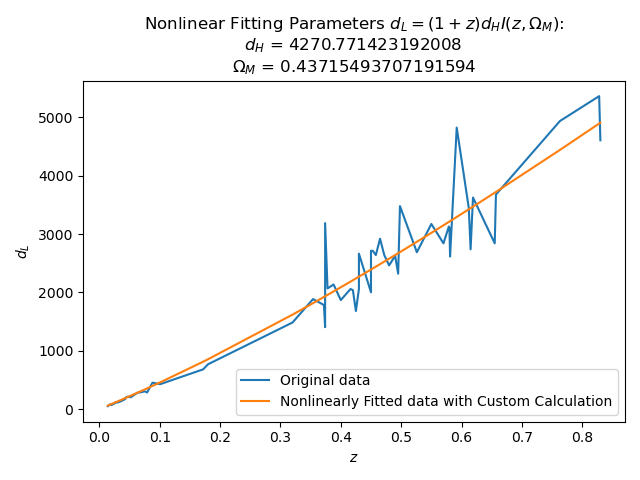
\includegraphics[width=\linewidth]{figures/nonlinfit.png}}
    \caption{Nonlinear Fit on the Data with Custom Method}
    \label{fig:nonlinfit}
    \end{figure}

\paragraph{} As a first guess of $d_H$, the result found from linear fit is used, and, for the first guess of $\Omega_M$, the value of $0.5$ is used. As a result, the below outcomes are obtained.
\begin{equation*}
    d_H = 4270.771
\end{equation*}

\begin{equation*}
    \Omega_M = 0.4371
\end{equation*}

\subsection{Error Estimation}
\paragraph{} For the error estimation, the seperate methods are followed. Firstly, usage of the \textit{Gaussian} distributions of the $d_L$ and its measurement errors are incorporated as explained in the \textit{Problem Set 4}. Secondly, the whole nonlinear curve fitting process is managed by the $SciPy$ built-in function, and its error estimations are observed.

\begin{figure}[H]
    \centerline{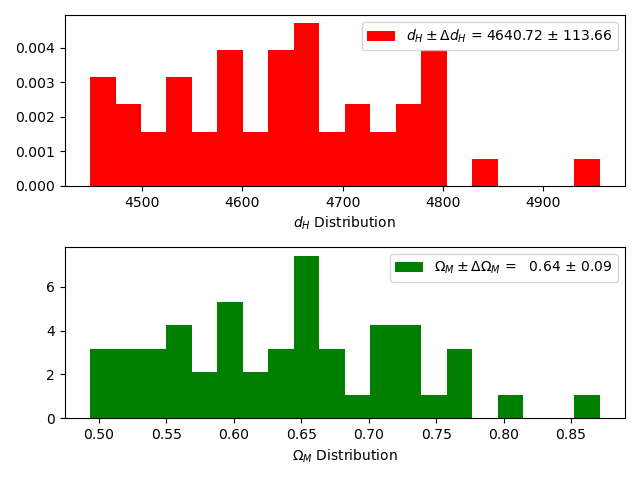
\includegraphics[width=\linewidth]{figures/dhomegadist.png}}
    \caption{Error Estimation using Gaussian Distributions}
    \label{fig:dhomegadist}
    \end{figure}
\paragraph{} Observing Figure \ref{fig:dhomegadist}, and Figure \ref{fig:dhomegadistcomp}, it can be concluded that the custom error estimation does not result in with a good accruacy as it can be encountered in the SciPy function case. However, it should be also noted that the custom error estimation gives a smaller uncertainty bound, which can be interpreted favourably. On the other hand, from the Figure \ref{fig:nonlinfit}, and Figure \ref{fig:nonlinfitscipy}, it should be concluded that the both models have a quiet good approximation performance.
\begin{figure}[H]
    \centerline{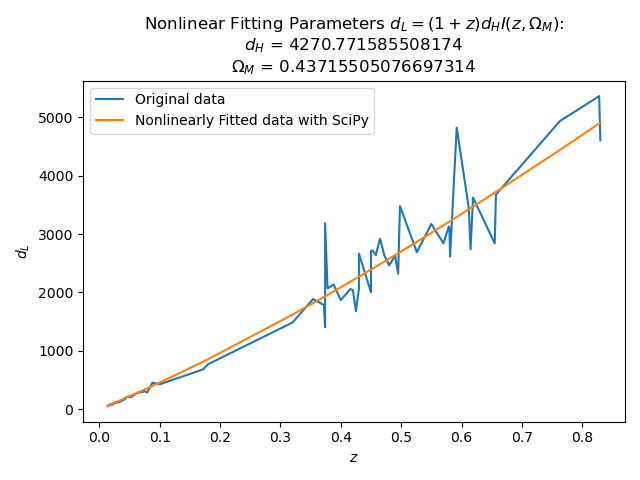
\includegraphics[width=0.8\linewidth]{figures/nonlinfitscipy.png}}
    \caption{Nonlinear Fit on the Data with SciPy Built-in Function}
    \label{fig:nonlinfitscipy}
    \end{figure}

\begin{figure}[H]
    \centerline{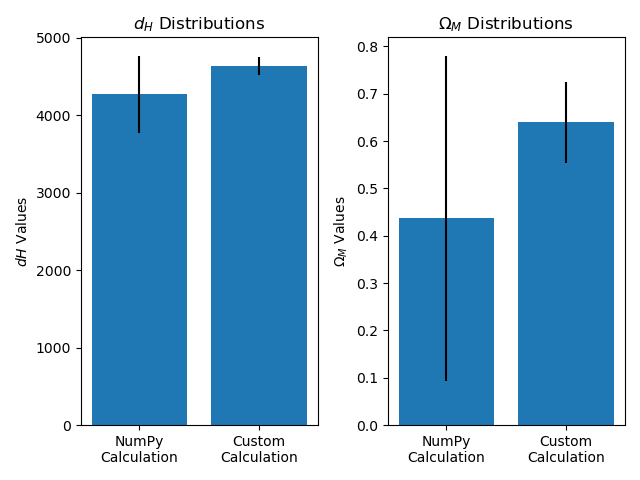
\includegraphics[width=0.7\linewidth]{figures/dhomegadistcomp.png}}
    \caption{Error Estimations using SciPy Built-in Method and its Comparison with Custom Method}
    \label{fig:dhomegadistcomp}
    \end{figure}
    

\section{Problem XII}
\paragraph{} In this problem, the subject function is the following:
\begin{equation*}
    f(x) = \frac{1}{1 + 25x^2}
\end{equation*}
\paragraph{}Above function was being tried to approximate via using various methods, and the performance of the approximation was calculated via following metric called \textit{Frobenius norm}.
\begin{equation*}
    E(n) = \left[ \frac{1}{2} \int_{-1}^{1} \lvert R(x) - R_n(x)  \rvert ^2\right]
\end{equation*}
\subsection{Exact Polynomial Fit with Varying Number of Equidistant Nodes}
\label{sec:exactpoly}
\begin{figure}[H]
    \centerline{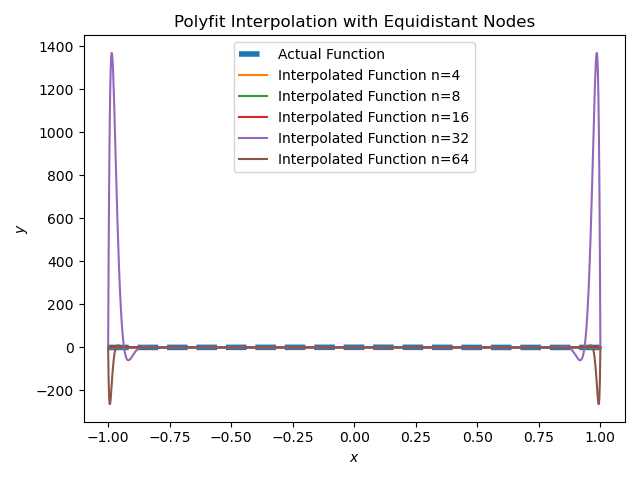
\includegraphics[width=\linewidth]{figures/poly.png}}
    \caption{Exact Polynomial Fit with Varying Number of Equidistant Nodes}
    \label{fig:poly}
    \end{figure}
\paragraph{} From Figure \ref{fig:poly} and Figure \ref{fig:frobpoly} it can be observed that the increase in the number of nodes does not result in the increase of the quality. It can be explained by the \textit{Runge's phenomenon}, which basically tells that the increase in the number of equidistant nodes doe not necessarily result in the increase of accuracy. From Figure \ref{fig:frobpoly}, it can be seen that the Frobenius norm is tend to decrease, however, Figure \ref{fig:poly} clearly shows that it is not an logical approximation. 


\begin{figure}[H]
    \centerline{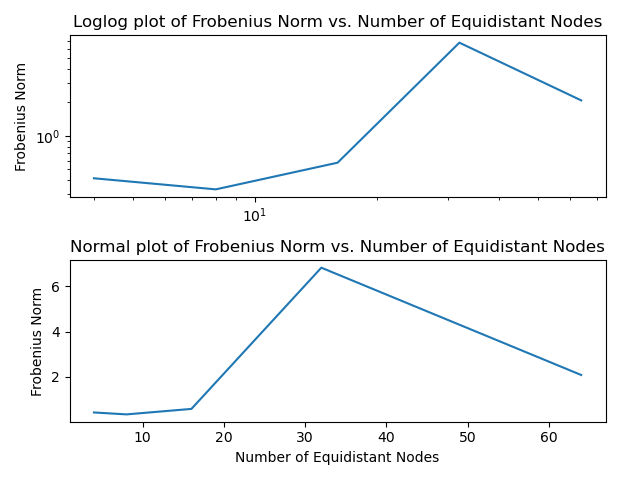
\includegraphics[width=\linewidth]{figures/frobpoly.png}}
    \caption{Frobenius Norm of Exact Polynomial Fit with Varying Number of Equidistant Nodes}
    \label{fig:frobpoly}
    \end{figure}
        

\subsection{Linear and Cubic Spline Interpolation}
\paragraph{} In this section, the spline interpolation will be discussed. From Figure \ref{fig:linspline} and Figure \ref{fig:froblinspline}, even linear spline interpolation does result in good approximation. The basic result behind that might be the fact that it is most basic thing one can come up with to approximate a function, like connecting the dots. However, the downside is the fact that this approximation yields a huge number of sharp points due to the piecewise line connections. These sharp points may result in undesirable derivative expression at there.

\begin{figure}[H]
    \centerline{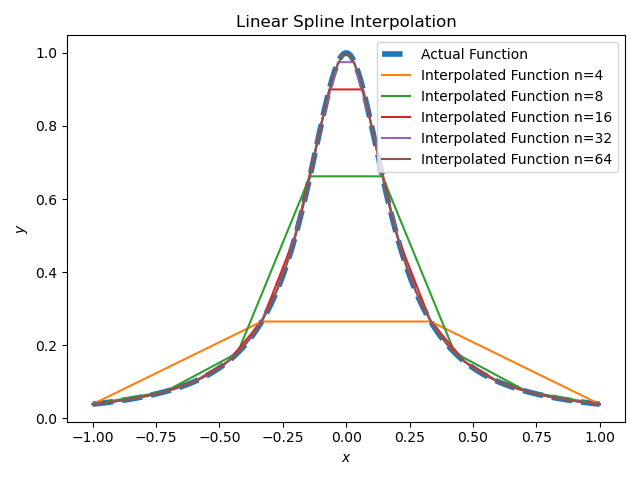
\includegraphics[width=0.8\linewidth]{figures/linspline.png}}
    \caption{Linear Spline Interpolation on the Data}
    \label{fig:linspline}
    \end{figure}

\begin{figure}[H]
    \centerline{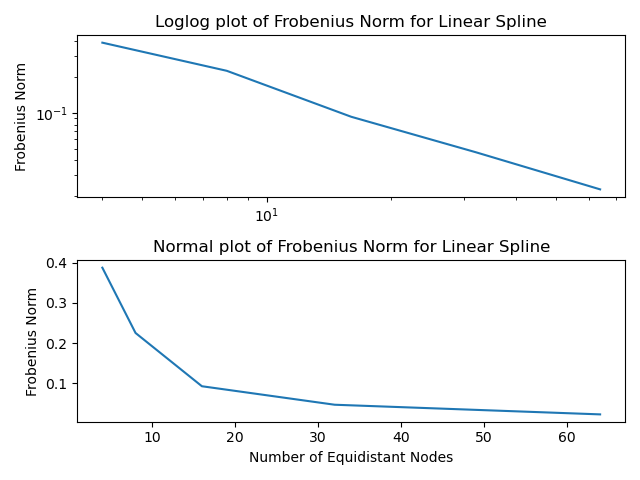
\includegraphics[width=0.7\linewidth]{figures/froblinspline.png}}
    \caption{Frobenius Norm of the Linear Spline Interpolation on the Data}
    \label{fig:froblinspline}
    \end{figure}

\paragraph{} In Figure \ref{fig:cubspline} and Figure \ref{fig:frobcubspline}, the cubic spline interpolation results can be investigated. In linear spline interpolation, the sharpness of the result was discussed. In this sense, the cubic spline interpolation can be thought as a solution to that problem. The cubic spline interpolation succesfully manages to connect nodes without losing the continuity.

\begin{figure}[H]
    \centerline{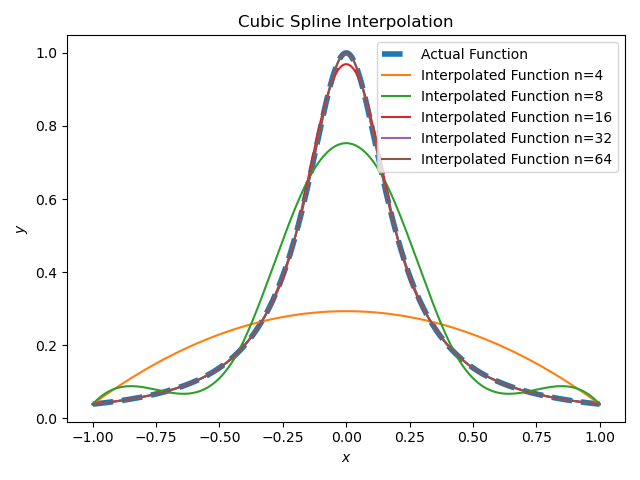
\includegraphics[width=\linewidth]{figures/cubspline.png}}
    \caption{Cubic Spline Interpolation on the Data}
    \label{fig:cubspline}
    \end{figure}
Therefore, in the the context of differentiability, the more desired results are obtained.
\begin{figure}[H]
    \centerline{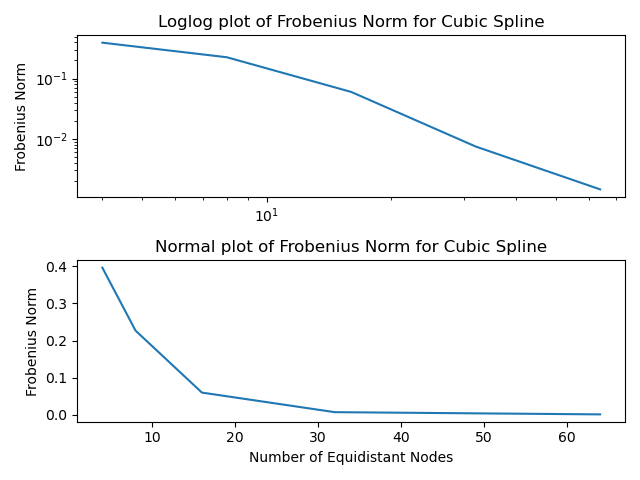
\includegraphics[width=\linewidth]{figures/frobcubspline.png}}
    \caption{Frobenius Norm of the Cubic Spline Interpolation on the Data}
    \label{fig:frobcubspline}
    \end{figure}

\subsection{Exact Polynomial Fit with Chebyshev Nodes}

\paragraph{} In Section \ref{sec:exactpoly}, it was discussed that the increase in the number of Equidistant nodes does not result in the performance increase. However, there is a way to fix it. The usage of the not-equidistant nodes can somehow yield more efficient results. The one convention as a not-equidistant node distribution is the usage of the \textit{Chebyshev nodes}. Chebyshev nodes can be defined as a projection of equidistant points on a unit circle. From Figure \ref{fig:polycheby}, one can observe that the usage of the \textit{Chebyshev nodes} immediately brings more satisfying approximations.
\begin{figure}[H]
    \centerline{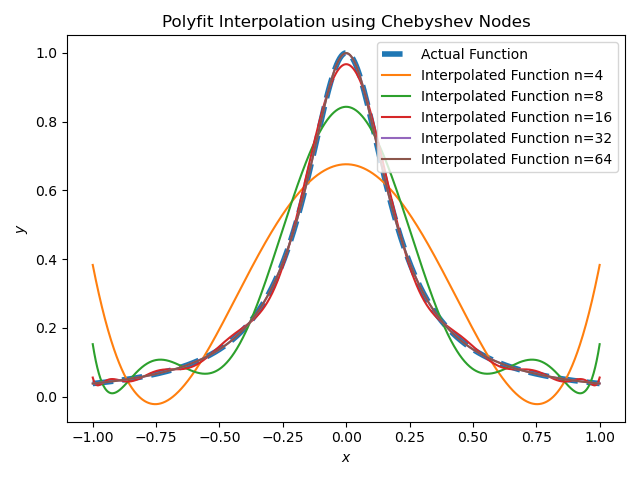
\includegraphics[width=0.8\linewidth]{figures/polycheby.png}}
    \caption{Exact Polynomial Fit with Chebyshev Nodes}
    \label{fig:polycheby}
    \end{figure}
\paragraph{} Moreover, having observed Figure \ref{fig:frobpolycheby}, the decrease in the Frobenius norm can be easily detected.
\begin{figure}[H]
    \centerline{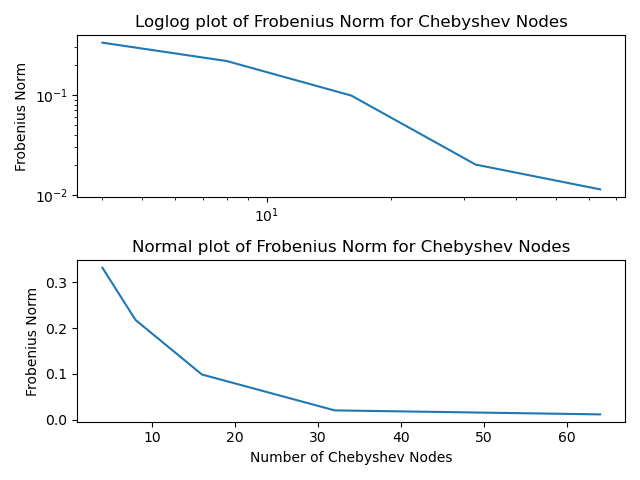
\includegraphics[width=0.7\linewidth]{figures/frobpolycheby.png}}
    \caption{Frobenius Norm of the Exact Polynomial Fit with Chebyshev Nodes}
    \label{fig:frobpolycheby}
    \end{figure}
\subsection{Polynomial Fit when Number of Nodes is not Equal to Degree of Polynomial}

    
\begin{figure}[H]
    \centerline{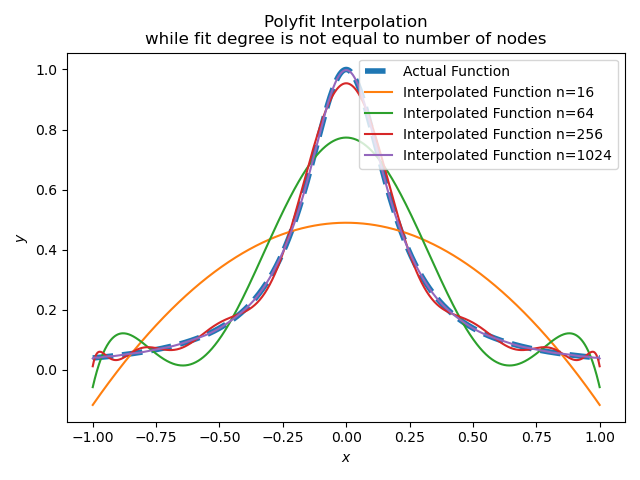
\includegraphics[width=\linewidth]{figures/polynenodes.png}}
    \caption{Polynomial Fit when Number of Nodes is not Equal to Degree of Polynomial}
    \label{fig:polynenodes}
    \end{figure}
     
\paragraph{} The final observation is the relation between the number of nodes and degree of fit. So far, for polynomial fitting, the number of nodes were equal to the degree of fitting. However, one should also observe the effect of the nonequality between them. In the all curves located on the Figure \ref{fig:polynenodes}, the following relation was followed:
\begin{equation*}
    Degree \; of \; Fitting = \sqrt{n} - 1
\end{equation*}

\paragraph{} According to the Figure \ref{fig:polynenodes}, one can easily deduct that although the number of nodes is climactic, the fitted lines manages to approximate well. This finding also can be verified by investigating the Figure \ref{fig:frobpolynenodes}, which clearly shows that although the number of nodes increases, the Frobenius norms insist on decreasing.
    
\begin{figure}[H]
    \centerline{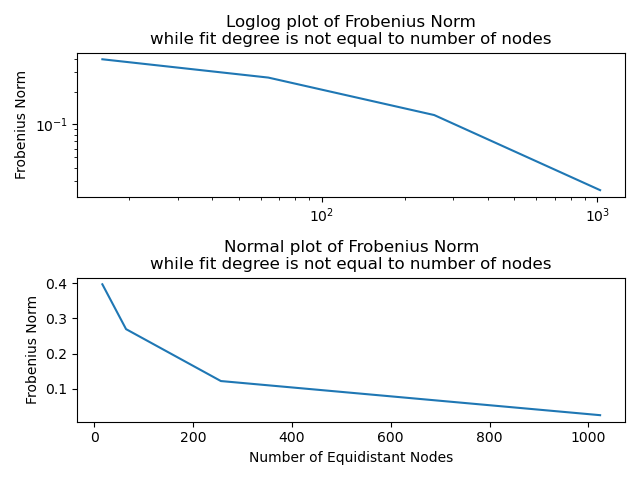
\includegraphics[width=\linewidth]{figures/frobpolynenodes.png}}
    \caption{Frobenius Norm of the Polynomial Fit when Number of Nodes is not Equal to Degree of Polynomial}
    \label{fig:frobpolynenodes}
    \end{figure}
    

    

    
    

\end{document}

              


